% 1. Einleitung
\section{Einleitung}

In der Vorlesung Informationspräsentation von Herrn Prof. Dr. Kretschmer ist
ein Projekt als Prüfungsleistung vorgesehen. Um diese Leistung nachzuweisen,
haben wir, Hong Phuc Hobui und Ragnar Bonk, diese kleine Silverlight-Anwendung
realisiert. Sie kann die Arbeitsweise beliebiger endlicher deterministischer
Automaten (DEA) mit beliebiger Eingabe animieren. Das vorliegende Dokument gibt
einen Überblick über die Funktionsweise und die wesentlichen Interna der
Anwendung.

%%%%%%%%%%%%%%%%%%%%%%%%%%%%%%%%%%%%%%%%%%%%%%%%%%%%%%%%%%%%%%%%%%%%%%%%%%%%%
% 2. Aufgabenbeschreibung
\section{Aufgabenbeschreibung}
Dieser Abschnitt beschreibt die Aufgabenstellung und somit die einzelnen
Anforderungen an die Anwendung. Diese Beschreibung basiert in weiten Teilen auf
der Original-Aufgabenbeschreibung von Herrn Kretschmer.

%2.1 Vorbereitung
\subsection{Vorbereitung}
Die Silverlight-Anwendung liest aus einer XML-Datei die Beschreibung eines DFA
und stellt diesen als Graph dar. Der Name der XML-Datei wird vom Benutzer
angegeben. Der Benutzer kann jederzeit zu einem anderen Automaten wechseln,
indem er dessen XML-Datei einliest. 

Der Benutzer kann ein Eingabewort eingeben und dann die Animation starten. Dies
kann er beliebig oft wiederholen. 

%2.2 Animation
\subsection{Animation}
Das Eingabewort wird stets komplett angezeigt. Dabei werden aber die bereits
verarbeiteten Zeichen, das aktuelle Zeichen und die noch zu verarbeitenden
Zeichen optisch anders dargestellt. 

Der aktuelle Zustand wird optisch hervorgehoben. 

Die Animation erfolgt zeichenweise wie folgt: Das aktuelle Zeichen bewegt sich
aus dem Eingabewort in den aktuellen Zustand, bewegt sich \glqq{}suchend\grqq{}
in diesem Zustand und verlässt über einen passenden Übergang den aktuellen
Zustand und bewegt sich in den Folgezustand, der dadurch zum aktuellen Zustand
wird. Das Zeichen verschwindet dann. Gibt es keinen passenden Übergang, wird
dies optisch signalisiert und die Animation ist beendet. Ist das Wort
abgearbeitet, so wird das Ergebnis (akzeptieren oder verwerfen) schriftlich und
optisch angezeigt. 

%2.3 Beschreibungsdatei
\subsection{Beschreibungsdatei\label{sec:2:3}}
Die Beschreibungsdatei ist im XML-Format. Die Elemente der Beschreibungsdatei
haben folgende Bedeutung:

{\footnotesize
\begin{table}[H]\centering
\begin{tabular}{|l|l|l|}\hline
XML-Element     & Bezeichnung (deutsch) & Bedeutung      \\ \hline \hline
FiniteAutomaton & Endlicher Automat     & Wurzelelement  \\ \hline
InputAlphabet   & Eingabealphabet       & 
	\begin{minipage}{0.5\textwidth}
		Das Alphabet besteht aus den enthaltenen Symbolen.\vspace{0.5ex}
	\end{minipage}\\ \hline
Symbol         & Symbol (Zeichen)      &
	\begin{minipage}{0.5\textwidth}
		Der enthaltene String besteht aus einem Zeichen und ist ein Symbol des
		umfassenden Alphabets. Der String darf keinen Blank enthalten.
		\vspace{0.5ex}
	\end{minipage}\\ \hline
States         & Zustände              &
	\begin{minipage}{0.5\textwidth}
		Enthält genau einen Startzustand und beliebig viele sonstige Zustände,
		wobei es einen oder mehrere Endzustände gibt.
		\vspace{0.5ex}
	\end{minipage}\\ \hline
State          & Zustand               &
	\begin{minipage}{0.5\textwidth}
		Der String ist der Name des Zustandes.

		Das optionale Attribut \texttt{start} kann die Werte \texttt{Y} (yes) oder 
		\texttt{N} (no)
		haben. Es gibt an, ob der Zustand ein Startzustand ist oder nicht. Wenn
		es fehlt, ist der Wert \texttt{N}.

		Das optionale Attribut \texttt{accept} kann die Werte \texttt{Y} (yes) 
		oder \texttt{N} (no)
		haben. Es gibt an, ob der Zustand ein Endzustand ist oder nicht. Wenn
		es fehlt, ist der Wert \texttt{N}.

		Achtung: Ein Startzustand kann gleichzeitig Endzustand sein.
		\vspace{0.5ex}
	\end{minipage}\\ \hline
Transitions    & Übergänge            &
	\begin{minipage}{0.5\textwidth}
		Enthält beliebig viele Übergänge.

		Der beschriebene Automat ist deterministisch
		\vspace{0.5ex}
	\end{minipage}\\ \hline
Transition     & Übergang             &
	\begin{minipage}{0.5\textwidth}
		Das Attribut \texttt{from} ist der aktuelle Zustand, \texttt{to} ist der neue
		Zustand, \texttt{symbol} ist das aktuelle Eingabezeichen.
		\vspace{0.5ex}
	\end{minipage}\\
\hline
\end{tabular}
\end{table}
}

%2.3.1 Beispiel einer Eingabedatei.
\subsubsection*{Beispiel einer Eingabedatei}
\setmonofont[Scale=0.75]{Inconsolata}
\begin{multicols}{2}
\begin{minted}[tabsize=4]{xml}
<?xml version="1.0" encoding="ISO-8859-1"?> 
<!-- Hopcroft/Motwani/Ullman S. 60 --> 
<FiniteAutomaton> 
  <InputAlphabet> 
    <Symbol>0</Symbol> 
    <Symbol>1</Symbol> 
  </InputAlphabet> 
  <States> 
    <State start="Y" accept="Y">q0</State> 
    <State>q1</State> 
    <State>q2</State> 
    <State>q3</State> 
  </States> 
  <Transitions> 
    <Transition from="q0" symbol="0" to="q2" /> 
    <Transition from="q0" symbol="1" to="q1" /> 
    <Transition from="q1" symbol="0" to="q3" /> 
    <Transition from="q1" symbol="1" to="q0" /> 
    <Transition from="q2" symbol="0" to="q0" /> 
    <Transition from="q2" symbol="1" to="q3" /> 
    <Transition from="q3" symbol="0" to="q1" /> 
    <Transition from="q3" symbol="1" to="q2" /> 
  </Transitions> 
</FiniteAutomaton> 
\end{minted}
\end{multicols}
\setmonofont[Scale=0.90]{Inconsolata}


%%2.4 Implementierung
\subsection{Implementierung}
Das Programm muss in Silverlight geschrieben sein.

%2.5 Dokumentation
\subsection{Dokumentation}
Es ist eine kurze (5-10 Seiten) Dokumentation anzufertigen. Diese sollte
insbesondere die Architektur und Funktionsweise des Programms beschreiben.
Ebenfalls sollte die Installation des Programms erläutert werden. Bei der
Installation ist darauf zu achten, dass keine absoluten Pfadangaben
vorausgesetzt werden. 

%3. Realisierung
\section{Realisierung}
Im ersten Moment hört es sich an, als ob die Aufgabenbeschreibung und
Silverlight (in Zusammenarbeit mit Expression Blend) optimal zueinander passen
würden. Während der Realisierung hat sich jedoch herausgestellt, dass es
dennoch einige typische, wie z.B. Koordinaten-Umrechnung, aber auch unerwartete
Hürden und Probleme gab. Wären wir erfahrene Silverlight-Entwickler, wäre das
eine oder andere davon sicher eine leichte Übung gewesen. Dennoch haben wir uns
den Herausforderungen gestellt und und uns iterativ immer weiter an die Lösung
herangearbeitet. Dieser Abschnitt zeigt einige der Probleme und deren Lösung
auf.

%3.1 Eingabe-XML
\subsection{Eingabe-XML}
Bereits beim Verarbeiten des Eingabe-XML traten erste Probleme auf. Die
vorgeschlagene Struktur der Eingabe-Datei als auch die restliche
Aufgabenbeschreibung macht keine Angaben darüber, wie die einzelnen Knoten zu
positionieren sind. Demnach hätte man eigentlich eine automatische Routine zum
Positionieren der Knoten schreiben müssen. Hiermit wäre dann aber auch direkt
die Anforderung verbunden gewesen, den Graphen möglichst planar zu zeichnen.

Sicherlich sind uns hierfür die Lösungsansätze aus unserem Studium bekannt, wie
z.B. das topologische Sortieren. Allerdings hätte dies einen deutlichen
Mehraufwand bedeutet. Deswegen wurde nach Absprache mit Herrn Kretschmer
beschlossen, dass der Fokus stärker auf der Animation als auf einem
automatischen Layout des Graphen liegen soll. D.h., dass das Eingabe-XML derart
erweitert wird, dass die Position der einzelnen Knoten bereits dort bestimmt
wird:

\begin{table}[H]
	\centering
	\begin{tabular}{|l|l|l|}\hline
XML-Element & Bezeichnung (deutsch) & Bedeutung \\ \hline
State       & Zustand               & 
\begin{minipage}{0.5\textwidth}
		Zu den oben bereits genannten Attributen werden zwei weitere, obligatorische
		hinzugefügt: \texttt{x} und \texttt{y}. Sie geben die (Bildschirm-) Koordinaten des Knotens
		an.\vspace{1ex}
	\end{minipage}\\ \hline
\end{tabular}
\end{table}

Ein weiteres Problem mit dem Lesen des Eingabe-XMLs war die Validierung. Denn
Eingabe-Daten müssen i.d. R. immer erst geprüft werden, bevor sie in
irgendeiner Weise verwendet werden. Ausnahmen hiervon sind möglich, wenn
sichergestellt ist, das die Eingabe-Daten immer gültig sind.

Daher sollte nach ersten Plänen die Eingabe-Datei mittels XML-Schema validiert
werden. Doch Nachforschungen diesbezüglich ergaben, dass Silverlight eine
Schema-Validierung wohl nur serverseitig unterstützt, clientseitig ist
lediglich DTD verfügbar. Und dies obwohl Silverlight selbst sehr stark auf
XML-Techniken basiert.

Die Lösung hierfür war ebenfalls eine Absprache mit Herrn Kretschmer: Es wurde
festgelegt, dass davon ausgegangen werden darf, dass die Eingabe-Dateien immer
korrekt sind.

Der Code für das Einlesen der Eingabe-Datei liegt in der Klasse \texttt{XmlParser.cs}.

%3.2 Darstellen des Graphen
\subsection{Darstellen des Graphen}
An dieser Stelle traten die wohl ganz typischen Probleme der grafischen
Programmierung auf: Das Umrechnen der Bildschirmkoordinaten in das kartesische
Koordinatensystem.

Denn obwohl es vermeintlich so aussieht, als könne man mit Expression Blend
einen DFA in ein paar Minuten zusammen klicken, dem ist nicht so: Einen
Automaten hat man mit Expression Blend zwar sicherlich innerhalb dieser Zeit,
dennoch wäre dieser dann hinsichtlich seiner Funktionsweise und Eingabe
beschränkt.

Interessanterweise hat offenbar auch Silverlight diesbezüglich kein
einheitliches und einfach zu nutzendes Konzept: In Java z.B. basieren die
Methoden zum Zeichnen einer Linie auf dem Koordinatensystem des Bildschirms.
Die mathematischen Grundfunktionen (wie z.B. Sinus) legen allerdings wieder das
kartesische System zugrunde. Dies ist in Silverlight nicht anders.

Die Umrechnung (mathematisch gesehen) ist zwar nicht so schwierig, aber
aufwändig und wir mussten nur für diesen Zweck, eigens Klassen konzipieren,
implementieren und testen. Und dies nicht nur für das Positionieren der Knoten,
sondern auch für das Darstellen der Pfeile der Übergänge. Also schufen wir
Klassen für diese Aufgaben:

\begin{description}
	\item{\texttt{EPoint} (in \texttt{Cartesian.cs})}: 
		Stellt einen kartesischen Punkt dar und enthält z.B.  die Methoden
		\texttt{transformCoordinate()} bzw. \texttt{rotateCoordinate()}.

	\item{\texttt{EVector} (in \texttt{Cartesian.cs})}: Stellt einen Vektor im
			kartesischen System mit den relevanten Methoden dar.

	\item{\texttt{LayoutComputer.cs}}: Dient zum Berechnen der Knoten bzw. Kanten.
	\item {\texttt{GraphDrawer.cs}}: Benutzt die von den oben genannte Klassen
		ermittelten Informationen um den Graphen (Automaten) zu zeichnen.
\end{description}
%3.3 Planen und Durchführen der Animation
\subsection{Planen und Durchführen der Animation}

\subsubsection{Verfahrensweise}
Zunächst ist klar, dass es für jeden Knoten grundsätzliche vier verschiedene
mögliche Animationen gibt:

\begin{description}
	\item[\texttt{Senden}] Suchen der nächsten passenden Kante für das aktuelle Eingabesymbol.
	\item[\texttt{Empfangen}] Wenn ein Zeichen von einem anderen Knoten (über eine
		gültige Kante) gesendet wurde, so wird es \glqq{}empfangen\grqq{}. Dies wird dann
		dementsprechend animiert.
	\item[\texttt{Akzeptieren}] Wenn die Eingabe komplett gelesen ist und der aktuelle
		Zustand ein Endzustand ist.
	\item[\texttt{Verwerfen}] Alles Andere fällt in diese Kategorie und wird mit einer ablehnenden
		Animation quittiert.
\end{description}

Somit war die Idee für das Ausführen der Animation eigentlich, die
Eingabe-Datei einzulesen, jeden Knoten (\texttt{State}) zu parsen, anzuzeigen und
jedem Knoten für jeden dieser Fälle eine (eigene) Animation zuzuweisen. Jeder
Knoten sollte dann von seinem Vorgänger benachrichtigt werden, welches Symbol
gesendet wurde und sollte dann die passende Animation einem (globalen)
Storyboard zuweisen. Dieses sollte dann abgespielt werden und die
entsprechenden Features wie Stoppen, Spulen usw. bieten. Demnach hätte dann ein
einziges Storyboard zum Abspielen der gesamten Animation für ein Eingabewort
existiert. Ein Spulen innerhalb dieser Art der Wiedergabe wäre (vermutlich)
problemlos möglich gewesen.

Es hat sich jedoch herausgestellt, dass pro Storyboard und Objekt nur eine
Animation pro  Eigenschaft registriert werden darf. D.h. dass nur eine
Animationen (Veränderung) der Objekt-Eigenschaft \texttt{width} des Objektes \texttt{A}
innerhalb eines Storyboards passieren darf.  \texttt{width} dürfte nur erhöht oder
verringert werden. Sind die Animationen auf verschiedene Eigenschaften (z.B. \texttt{x}-
und danach  \texttt{y}-Koordinate) verteilt, gibt es keine Probleme. Allerdings schränkt
dies die Möglichkeiten stark ein: Wenn die Animation für das Senden z.B. eine
Veränderung der \texttt{x}-Koordinate beinhaltet hat, so konnte die für das Empfangen
diese Koordinate nicht mehr nutzen.

Unsere Lösung sieht also anders aus: Es gibt einzelne Storyboards für jede der
oben genannten Animationen und jeder Knoten (\texttt{VisualNode.cs}) hat seine eigenen
Instanzen davon. Außerdem bietet das Storyboard die Möglichkeit eine
\texttt{Callback}-Funktion aufzurufen, wenn die Animation beendet ist. Dadurch kann ein
Storyboard bei seinem Ende den Nachfolger starten. Dasselbe gilt im übrigen
auch für die Kanten (\texttt{VisualEdge.cs}).

Nun gibt es noch eine Liste, welche die durchzuführenden Animationen
beinhaltet. Diese Liste wird erstellt, in dem ein Algorithmus den Automaten
passend zur Eingabe simuliert.Das Ergebnis steht also schon vor Animationsstart
fest auch wenn dies nicht sichtbar geschieht. Der Algorithmus ist in der Klasse
\texttt{AnimationPlanner.cs} implementiert.

%3.3.1 'Stepline' und 'Flowing input'
\subsubsection{\guielement{Stepline} und \guielement{Flowing input}\label{sec:3:3:1}}

Zwei Besonderheiten sollen noch erwähnt werden. Da Kinder einen Namen brauchen,
haben wir sie \texttt{Stepping} und \texttt{Flowing input} genannt.

\begin{description}
	\item [\guielement{Stepline}] Durch die oben verwendeten
		\texttt{Callback}-Funktionen und ein paar passende Zeilen Code ist es
		möglich, den Automaten zu pausieren, also die Animationsabfolge zu
		unterbrechen. Über das Bedienelement \texttt{Stepline} kann nun
		\glqq{}gespult\grqq{} werden, einzelne Storyboards sind dadurch direkt
		wählbar. Startet man die Animation nun wieder, so wird sie ab dem
		selektierten Storyboard fortgesetzt.

	\item [\guielement{Flowing input}] Dies ist die Animation der \glqq{}fallenden\grqq{}
		Eingabesymbole, welche durch das Bedienelement \guielement{Flowing input}
		aktiviert werden kann. Leider gibt es hier ein paar
		Synchronisationsprobleme weswegen bei der Verwendungen dieser Option
		die \texttt{Stepline} deaktiviert ist.
\end{description}

%3.4 Architektur
\subsection{Architektur}

Die Anwendung folgt in weiten Teilen der Silverlight-Vorgabe, dass GUI-Elemente
in XAML und der Rest in Programmcode (\verb:C#:) geschrieben wird. So
beherbergt die Klasse \texttt{MainPage.xaml} den Grundaufbau des Automaten. Die
XAML-Definitionen für die Knoten liegen in \texttt{Visual*NodeGrid.xaml}, diejenigen für
die Kanten in \texttt{VisualEdgeGrid.xaml} und die für die Eingabe (bei Verwendung von
\texttt{Flowing input}) letztendlich in \texttt{VisualInputGrid.xaml}.

%5. Installation
\section{Installation}


Eine Installation ist nicht erforderlich. Das Programm kann unter
\url{http://wanderer.site50.net/SilverlightApplication6.html} mit einem Browser
ausprobiert werden. Voraussetzung dafür ist aber eine Silverlight-Version >=
4.0.50826.0. Der Quellcode ist ebenfalls online verfügbar und zwar unter
\url{http://code.google.com/p/silverlight-dfa/}. Zum Öffnen des Projektes ist
allerdings Microsoft Visual Studio 2010 mit Service Pack 1 (bzw. Silverlight
Developer Tools 4) erforderlich.

%6. Bedienung
\section{Bedienung}

Grundsätzlich gilt erst mal, dass Bedienelemente, deren Nutzung im aktuellen
Zustand des Programmes nicht sinnvoll oder möglich ist, deaktiviert sind. Sie
werden dann freigeschaltet, wenn die Bedingungen für ihre Nutzung erfüllt sind.

Nach dem Start sieht die Anwendung zunächst aus, wie in Abbildung \ref{fig:gui}. Die
Anwendung hat zu diesem Zeitpunkt automatisch einen integrierten
Beispielgraphen geladen.

\begin{figure}[H]
	\centering
	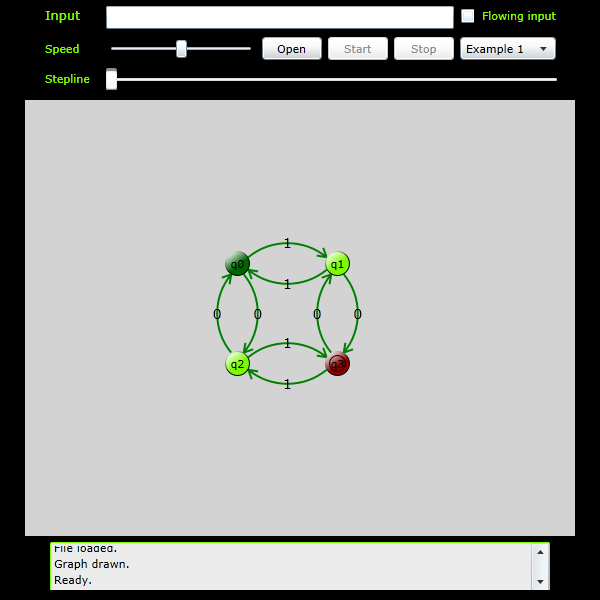
\includegraphics[scale=0.65]{gui.png}
	\caption{\label{fig:gui} Nach dem Start der Anwendung}
\end{figure}

Um andere Graphen zu Laden gibt es zwei verschiedene Möglichkeiten:
\begin{enumerate}
	\item Im Drop-Down-Menü ganz rechts, in welchem am Anfang \guielement{Example 1}
		ausgewählt ist, können weitere, integrierte Beispiele geladen werden.

	\item Über den \guielement{Open}-Button können eigene Graphen aus dem lokalen Dateisystem
		geladen werden. Diese müssen dann das unter \ref{sec:2:3} beschriebene Format haben.
\end{enumerate}

Hat man sich für einen Graphen entschieden, sollte zunächst überlegt werden, ob
die Option \guielement{Flowing input} (siehe \ref{sec:3:3:1}) verwendet werden soll. Ist dies der
Fall, so sollte nun die entsprechende Checkbox aktiviert werden.

Soll die Abspielgeschwindigkeit verringert oder erhöht werden, so kann dies
ebenfalls jetzt eingestellt werden.

Wurden alle Einstellungen vorgenommen, kann in das Eingabefeld (\guielement{Input}) nun
ein Wort des Eingabealphabets eingetippt werden. Symbole, die nicht im
Eingabealphabet definiert wurden, können nicht eingegeben werden.

Ein Klick auf den \guielement{Start}-Button bringt nun die Animation zur Ausführung.

Viele Bedienelemente sind während der Ausführung der Simulation nicht
verfügbar. Soll die Animation angehalten werden, so kann der
\guielement{Stop}-Button betätigt werden. Wurde auf die Verwendung von
\guielement{Flowing input} verzichtet, so kann nun über die
\guielement{Stepline}-Leiste \glqq{}gespult\grqq{} werden (siehe
\ref{sec:3:3:1}). Soll \guielement{Flowing input} nun (de-)aktiviert werden, so
muss zunächst die komplette Eingabe gelöscht werden.

Statusnachrichten der Anwendung können die ganze Zeit über in der grauen
\guielement{Logbox} ganz unten verfolgt werden.
